\documentclass[preprint,12pt]{revtex4}
\usepackage{grffile}%so the file kind is the last .*
\usepackage{bm} %for bold math
\usepackage{amsmath,mathrsfs}
\usepackage{amssymb}
\newcommand{\op}[1]{{\hat{\mathcal#1}}}
%\AtEndDocument{\message{^^JLaTeX Info: Executing hook `AtEndDocument'.}}
\def\colore{red}
\usepackage[usenames,dvipsnames]{xcolor}
\usepackage{animate}
%%%% fancy header
\usepackage{fancyhdr}
\pagestyle{fancy}
\renewcommand{\headrulewidth}{2pt}
%%%%%
\usepackage[spanish,english]{babel}
\usepackage[utf8]{inputenc}
\usepackage{showlabels}
\usepackage{graphicx}
\usepackage{fancyvrb}
%%%%*****************%%%% fine hyperef 
\usepackage[backref,pdffitwindow,colorlinks,citecolor={red},linkcolor={blue}]{hyperref}
%%%%*****************%%%%
% Definitions 
%%%%% defs
%%%% acronimos
\def\acu{Accu-Check\textsuperscript{\textregistered}~Performa}
\def\goni{Glucometro \'Optico No Invasivo}
\def\Reg{\textsuperscript{\textregistered}}
\def\tiniba{ TINIBA\textsuperscript{\textregistered}}
\def\gw{{\it GW}}
\def\gsa{Generaci\'on del Segundo Arm\'onico}
\def\shg{Second Harmonic Generation}
\def\sfg{Sum Frequency Generation}
\def\sdf{Generaci\'on de Suma de Frecuencias}
%%%%% accent of i
\def\'#1{\if#1i{\accent19\i}\else{\accent19#1}\fi}
%%%%% compa\~nias
\def\micro{{\it Supermicro}}
\def\lufac{{\it LUFAC}}
%%%%% lugares
\def\lou{Laboratorio de \'Optica Ultrar\'apida}
\def\roma{Universidad de Roma II}
\def\tor{``Tor Vergata''}
\def\dti{Direcci\'on de Tecnolog\'{\i}a e Innovaci\'on}
\def\dfa{Direcci\'on de Formaci\'on Acd\'emica}
\def\dg{Direcci\'on General}
\def\da{Direcci\'on Administrativa}
\def\ifug{Insituto de F\'isica de la U. de Guanajuato}
\def\icf{Instituto de Ciencias F\'isicas}
\def\unam{Universidad Nacional Aut\'onoma de M\'exico}
\def\uguille{Universidad del Nordeste, Argentina}
\def\fotonica{Departamento de Fotonica}
\def\grupo{Propiedades \'Opticas de Nano-Sistemas, Interfases y Superficies}
\def\grupoa{PRONASIS}
%\def\grupo{Propiedades \'Opticas de Superficies e Interfases y Sistemas Nanosc\'opicos}
%\def\grupoa{POSISNA}
\def\di{Direcci\'on de Investigaci\'on}
\def\dfa{Direcci\'on de Formaci\'on Acad\'emica}
\def\cio{Centro de Investigaciones en \'Optica}
\def\ciod{Centro de Investigaciones en \'Optica, León, Guanajuato.}
\def\Conacyt{Consejo Nacional de Ciencia y Tecnolog\'ia}
\def\Concyteg{Consejo  de Ciencia y Tecnolog\'ia del Estado de Guanajuato}
\def\conacyt{CONACyT}
\def\concyteg{CONCyTEG}
\def\lagos{Centro Universitario de los Lagos}
\def\udeg{Universidad de Guadalajara}
\def\dinv{Direcci\'on de Investigaci\'on}
\def\dop{Department of Physics}
\def\uoft{University of Toronto}
\def\ua{University of Texas at Austin}
\def\icf{Instituto de Ciencias Físicas, UNAM, Cuernavaca}
%%%%% gente
%% grupo
\def\gabriel{Gabriel Ramos Ortíz}
\def\ramon{Ram\'on~ Carriles~ Jaimes}
\def\ramonm{Ram\acute{o}n~ Carriles~ Jaimes}
\def\enrique{Enrique~ Castro~ Camus}
\def\raul{Ra\'ul Alfonso V\'azquez Nava}
\def\raulm{Ra\acute{u}l~ Alfonso~ V\acute{a}zquez~ Nava}
\def\beto{Norberto~ Arzate~ Plata}
\def\bmsa{Bernardo S. Mendoza}
\def\bms{Bernardo~ Mendoza~ Santoyo}
%% alumnos
\def\cesar{C\'esar Castillo Quevedo}
\def\cabellos{Jos\'e Luis Cabellos Quiroz}
\def\tona{Tonatiuh Rangel Gordillo}
\def\temok{Juan Cuauhtemoc Salazar Gonz\'alez}
\def\adan{Luis Adan Mart\'inez Jim\'enez}
\def\sean{Sean Martin Anderson}
\def\reinaldo{Reinaldo Zapata Pe\~na}
%%% alumnos del grupo
%% enrique
%Maestria:
\def\jorgee{Jorge Alberto Caballero Mendoza}
\def\sofia{Sofía Carolina Corzo García}
\def\ruth{Ruth Julieta Medina López} 
%Doctorado: 
\def\juane{Juan Jes\'us S\'anchez S\'anchez}
%Licenciatura
\def\alma{Alma Gabriela González Patlán}
%(con Ramon): 
\def\sergioer{Sergio Augusto Romero Serv\'{\i}n}
%% Raul
%Maestria:
\def\enriquer{Enrique Arag\'on Navarro}%udg
\def\salomonr{Salom\'on Rodr\'{\i}guez Carrera}
\def\hectorr{H\'ector Santiago Hern\'andez}
\def\victor{Victor Manuel Villanueva Reyes}
%% Ramon
%Maestria:
\def\alfredora{Alfredo Campos Mej\'{\i}a}
%% Beto
%Doctorado
\def\noe{No\'e Gonz\'alez Baquedano}
%% otros
\def\liliana{Liliana Wilson Herr\'an}
\def\gerardo{Gerardo E. S\'anchez Garc\'{\i}a Rojas}
\def\amalia{Amalia Mart\'inez Garc\'{\i}a}
\def\nacho{Ing. José Ignacio Diego Manrique}
\def\tere{Teresita del Niño Jesús Pérez Hernández}
\def\elder{Elder de la Rosa Cruz}
\def\gonzalo{Gonzalo P\'aez Padilla}
\def\wlm{W. Luis Moch\'an Backal}
\def\oracio{Oracio C. Barbosa Garc\'ia}
\def\hector{H\'ector Hugo S\'anchez Hern\'andez}
\def\marco{Marco Antonio Escobar-Acevedo}
\def\gil{Alejandro Gil-Villegas Montiel}
\def\ernesto{Ernesto Carlos Cort\'es Morales}
\def\fms{Fernando Mendoza Santoyo}
\def\cuevas{Francisco Javier Cuevas de la Rosa}
\def\brenda{Brenda Esmeralda Matr\'inez Z\'erega}
\def\guille{Guillermo Ortiz}
\def\cesar{Cesar Castillo Quevedo}
\def\sipe{Prof. John Sipe}
\def\mike{Prof. Michael Downer}
\def\jems{Jorge Enrique Mej\'ia S\'anchez}
\def\lamon{Ram\'on Rodr\'iguez Vera}
\def\ldp{Luis de la Pe\~na}
\def\sole{Rodolfo Del Sole}
\def\lucia{Lucia Reining}
\def\sch{Schr\"odinger}
\def\Cuevas{Francisco J. Cuevas de la Rosa}
%%%%% categorias
\def\ita{Investigador Titular A}
\def\itb{Investigador Titular B}
\def\itc{Investigador Titular C}
\def\itd{Investigador Titular D}
\def\ite{Investigador Titular E}
\def\sr{Senior Researcher}
\def\iac{Investigador Asociado C}    
\def\alm{Alumno de Maestr\'ia}
\def\ald{Alumno de Doctorado}
\def\all{Alumno de Licenciatura}
\def\adei{Asistente de Investigaci\'on}
\def\sniIII{S.N.I. nivel III}
\def\sni{S.N.I.}
\def\cv{Currículum Vitae}
%%%%%% fonts
\def\tit{\sf}
\def\col{\sc}
\def\alu{\it} % for students
\def\cual{2$^{do}$}
\def\anno{2005}
\def\spe{\vspace{.12cm}}
%%%%%% cosas
\def\capa{capa-a-capa}
\def\espin{espintr\'onica}
\def\oespin{optoespintr\'onica}
\def\proyecto{Photon Assisted Spintronics}
\def\npro{48915}
\def\cvk{cv\mathbf{k}}
\def\cvkp{c'v'\mathbf{k}'}
%%%%%% revistas
\def\prb{Physical Review B}
\def\prl{Physical Review Letters}
\def\ol{Optics Letters}
\def\opn{Optics and Photonics News}
\def\pssc{physica status solidi (c)}
%%%%%%%%%%%%%%%%%%%%%%%%%%%%%%%%%%%%%%%
%%%%%% griegas
\def\ga{\alpha}
\def\gb{\beta}
\def\gga{\gamma}
\def\gGa{\Gamma}
\def\go{\omega}
\def\got{\tilde\omega}
\def\gO{\Omega}
\def\gr{{\rho}}
\def\ge{\epsilon}
\def\ve{\varepsilon}
\def\gd{\delta}
\def\gD{\Delta}
\def\gl{\lambda}
\def\gs{\sigma}
\def\gS{\Sigma}
\def\gbs{\overline{\sigma}}
%%%%%% griegas with tilde
\def\gta{\tilde{\alpha}}
\def\gtb{\tilde{\beta}}
\def\gtga{\tilde{\gamma}}
\def\gto{\tilde{\omega}}
\def\gtO{\tilde{\Omega}}
\def\gtr{\tilde{\rho}}
\def\gte{\tilde{\epsilon}}
\def\vte{\tilde{\varepsilon}}
\def\gtd{\tilde{\delta}}
\def\gtD{\tilde{\Delta}}
\def\gtl{\tilde{\lambda}}
\def\gts{\tilde{\sigma}}
\def\gtS{\tilde{\Sigma}}
%%%%%% romans with tilde
\def\bftr{\tilde{\mathbf{r}}}
\def\bftp{\tilde{\mathbf{p}}}
\def\bftv{\tilde{\mathbf{v}}}
\def\ta{\tilde{a}}
\def\tb{\tilde{b}}
\def\tr{\tilde{r}}
\def\tp{\tilde{p}}
\def\tV{\tilde{V}}
\def\tv{\tilde{v}}
%%
\newcommand{\ham}{\hat{\mathcal H}}
%%%%%% bra kets
\newcommand{\la}{\langle}
\newcommand{\ra}{\rangle}
\newcommand{\ket}[1]{| #1 \rangle}
\newcommand{\bra}[1]{\langle #1 |}
\newcommand{\braket}[2]{\langle {#1} | {#2} \rangle}
\newcommand{\ketbra}[2]{| {#1} \rangle {#1} \langle {#2} |}
\newcommand{\ave}[1]{\langle {#1} \rangle}
%%%%%% averages
\newcommand{\prom}[1]{\langle {#1} \rangle}
%%%%%% creation and annihilation operators
\newcommand{\oa}{\hat a^{\tiny\strut}}
\newcommand{\oad}{\hat a^\dagger}
\newcommand{\oadk}{\hat a^\dagger_{\mathbf k}}
\newcommand{\oak}{\hat a^{\tiny\strut}_{\mathbf k}}
\newcommand{\obd}[1]{\hat b^\dagger_{#1}}
\newcommand{\ob}[1]{\hat b^{\tiny\strut}_{#1}}
%%%%%% Caligraphic
\newcommand{\cala}{{\cal A}}
\newcommand{\calf}{{\cal F}}
\newcommand{\calg}{{\cal G}}
\newcommand{\cald}{{\cal D}}
\newcommand{\cale}{{\cal E}}
\newcommand{\bfcale}{{\mathbf{\cal E}}}
\newcommand{\bfcalp}{{\mathbf{\cal P}}}
\newcommand{\bfcalg}{{\mathbf{\cal G}}}
\newcommand{\calo}{{\cal O}}
\newcommand{\calp}{{\cal P}}
\newcommand{\calr}{{\cal R}}
\newcommand{\cals}{{\cal S}}
\newcommand{\calw}{{\cal W}}
\newcommand{\calbd}{\boldsymbol{\mathcal{\cal D}}}
\newcommand{\calbp}{\boldsymbol{\mathcal{\cal P}}}
\newcommand{\calbv}{\boldsymbol{\mathcal{\cal V}}}
\newcommand{\calbs}{\boldsymbol{\mathcal{\cal S}}}
%%%%%% mathematicla bold roman & greek
\newcommand{\mbf}[1]{\mathbf{#1}}
\newcommand{\mbg}[1]{\boldsymbol{\mathcal {#1}}}
\newcommand{\bfA}{\mathbf{A}}
\newcommand{\bfB}{\mathbf{B}}
\newcommand{\bfC}{\mathbf{C}}
\newcommand{\bfD}{\mathbf{D}}
\newcommand{\bfE}{\mathbf{E}}
\newcommand{\bfF}{\mathbf{F}}
\newcommand{\bfG}{\mathbf{G}}
\newcommand{\bfH}{\mathbf{H}}
\newcommand{\bfI}{\mathbf{I}}
\newcommand{\bfJ}{\mathbf{J}}
\newcommand{\bfK}{\mathbf{K}}
\newcommand{\bfL}{\mathbf{L}}
\newcommand{\bfM}{\mathbf{M}}
\newcommand{\bfN}{\mathbf{N}}
\newcommand{\bfP}{\mathbf{P}}
\newcommand{\bfR}{\mathbf{R}}
\newcommand{\bfS}{\mathbf{S}}
\newcommand{\bfT}{\mathbf{T}}
\newcommand{\bfU}{\mathbf{U}}
\newcommand{\bfV}{\mathbf{V}}
\newcommand{\bfW}{\mathbf{W}}
\newcommand{\bfX}{\mathbf{X}}
\newcommand{\bfY}{\mathbf{Y}}
\newcommand{\bfZ}{\mathbf{Z}}
\newcommand{\bfa}{\mathbf{a}}
\newcommand{\bfb}{\mathbf{b}}
\newcommand{\bfc}{\mathbf{c}}
\newcommand{\bfd}{\mathbf{d}}
\newcommand{\bfe}{\mathbf{e}}
\newcommand{\bff}{\mathbf{f}}
\newcommand{\bfg}{\mathbf{g}}
\newcommand{\bfh}{\mathbf{h}}
\newcommand{\bfi}{\mathbf{i}}
\newcommand{\bfj}{\mathbf{j}}
\newcommand{\bfk}{\mathbf{k}}
\newcommand{\bfn}{\mathbf{n}}
\newcommand{\bfp}{\mathbf{p}}
\newcommand{\bfq}{\mathbf{q}}
\newcommand{\bfr}{\mathbf{r}}
\newcommand{\bfs}{\mathbf{s}}
\newcommand{\bft}{\mathbf{t}}
\newcommand{\bfu}{\mathbf{u}}
\newcommand{\bfv}{\mathbf{v}}
\newcommand{\bfx}{\mathbf{x}}
\newcommand{\bfy}{\mathbf{y}}
\newcommand{\bfz}{\mathbf{z}}
\newcommand{\bfzero}{\mathbf{0}}
\newcommand{\bfone}{\mathbf{1}}
%
\newcommand{\bfgeta}{\boldsymbol{\eta}}
\newcommand{\bfSig}{\boldsymbol{\Sigma}}
\newcommand{\bfsig}{\boldsymbol{\sigma}}
\newcommand{\bfgS}{\boldsymbol{\Sigma}}
\newcommand{\bfgs}{\boldsymbol{\sigma}}
\newcommand{\bfga}{\boldsymbol{\alpha}}
\newcommand{\bfgb}{\boldsymbol{\beta}}
\newcommand{\bfge}{\boldsymbol{\epsilon}}
\newcommand{\bfgvare}{\boldsymbol{\varepsilon}}
\newcommand{\bfgg}{\boldsymbol{\gamma}}
\newcommand{\bfgG}{\boldsymbol{\Gamma}}
\newcommand{\bfgphi}{\boldsymbol{\phi}}
\newcommand{\bfgpsi}{\boldsymbol{\psi}}
\newcommand{\bfgD}{\boldsymbol{\Delta}}
\newcommand{\bfgPhi}{\boldsymbol{\Phi}}
\newcommand{\bfgPsi}{\boldsymbol{\Psi}}
\newcommand{\bfgxi}{\boldsymbol{\xi}}
\newcommand{\bfgchi}{\boldsymbol{\chi}}
\newcommand{\bfgnabla}{\boldsymbol{\nabla}}
\newcommand{\bfgnu}{\boldsymbol{\nu}}
\newcommand{\bfgmu}{\boldsymbol{\mu}}
\newcommand{\bfgrho}{\boldsymbol{\rho}}
\newcommand{\bfgRho}{\boldsymbol{\Rho}}
%%%%%% nabla
\newcommand{\nablak}{\frac{\partial}{\partial\mathbf{k}} }
%%%%%% ; derivative
\def\gk{{;\mathbf k}}
%%%%%% k derivative
\newcommand{\deriv}[2] {\frac{\partial {#1}} {\partial {#2} }}
%%%%%% prime for \sum
\def\prima{\strut^{_{'}}}
%%%%%% subindices
%\def\eti{n\bfk}
\newcommand{\eti}[1]{_{#1 \bfk}}
\newcommand{\etiup}[1]{_{#1 \bfk s}}
\newcommand{\etidn}[1]{_{#1 \bfk \bar{s}}}
%%%%% superindice to push down the subindex in greeks!
\def\pd{^{\strut}}
%%%%% gauges
\def\rde{$\bfr\cdot\bfE$~}
\def\rder{length-gauge}
\def\pda{$\bfp\cdot\bfA$~}
\def\vda{$\bfv\cdot\bfA$~}
\def\vdar{velocity-gauge}
%%%%% integral over k
\def\intk{\int\frac{d^3k}{8\pi^3}}
%%%%% roman indices
\def\rmi{\mathrm{i}}
\def\rmj{\mathrm{j}}
\def\rmk{\mathrm{k}}
\def\rml{\mathrm{l}}
\def\rmr{\mathrm{r}}
\def\rma{\mathrm{a}}
\def\rmb{\mathrm{b}}
\def\rmc{\mathrm{c}}
\def\rmv{\mathrm{v}}
\def\rmz{\mathrm{z}}
\def\rmx{\mathrm{x}}
\def\rmy{\mathrm{y}}
%%%%% 
%iave: C01243171 y 0124317111

%%%%%%%%%%%%%%%%%%%%%%%%
\renewcommand{\theenumi}{\arabic{enumi}}
\renewcommand{\theenumii}{.\arabic{enumii}}
\renewcommand{\theenumiii}{.\arabic{enumiii}}
%
\renewcommand{\labelenumi}{\arabic{enumi}}
\renewcommand{\labelenumii}{\arabic{enumi}.\arabic{enumii}}
\renewcommand{\labelenumiii}{\arabic{enumi}.\arabic{enumii}.\arabic{enumiii}}
%
\newcommand{\cita}{\addtocounter{enumii}{1}}
%\selectlanguage{spanish}
\usepackage{setspace}
\usepackage{lastpage}
\cfoot{Page~\thepage~of \pageref{LastPage}}
\lhead{}
\rhead{POMETAS}
\usepackage{pageslts}
\begin{document}

\begin{center}
\strut

\vspace{2cm}

Poor's Man Guide to 2D Metamaterial Optical Properties 
\vspace{2cm}


Based on Haydock's Scheme\\

\vspace{2cm}
by

\vspace{2cm} 
Samuel Pérez$^1$, Guillermo Ortiz$^2$, Bernardo Mendoza$^3$ 
and Luis Mochán$^1$
\vspace{2cm}

$^1$ICF, UNAM, Cuernavaca, México.\\
$^2$U. del Nordeste, Corrientes, Argentina.\\
$^3$\cio, León, México.

\vfill
We thank Liliana Wilson for her help in developing \verb=corre-3g.pl=
and \verb=arrows.pl=
\end{center}
\newpage

\tableofcontents
\section{For the Impatiente}

In Sec.~\ref{sec:example} you'll find an example that cuts through the
chase, and perhaps this is where you should start, if you have read at
least once this manual.

\section{Introduction} 
These are the steps to be followed in order to calculate the optical
properties of a 2D binary metamaterial, characterized by $\ge_a(\go)$
and $\ge_{b}(\omega)$. Here $a$ represents the host material and $b$ the
inclusion, that could have any shape.

\textcolor{red}{Warning: So far it works for $\ge_b$ a complex/real number and
  $\ge_a$ a complex/real number or a file. For vacuum filled
  inclusions, chose $\ge_b=1.01$ and NOT $\ge_b=1$.} 

\textcolor{red}{Warning: Give the name of the dielectric functions
  as:}
\begin{itemize}
\item If a file: \verb=eps_name.dat=, where
 \verb=name= is the name of the element or material. \verb=name= is
 used by the scripts, so is very importnat to have this nomenclature. 
\item If a number: \verb=R+i*I=, where
 \verb=R= is the real part and \verb=I= is the imaginary part. Either
 one could be positive or negative.
\end{itemize}
Glossary:
\begin{itemize}
\item \verb=WD=: is the Working Directory. 
Try to use a nemotecnic
  name, for instance, making reference to the shape of the inclusion.  
\item 
\verb=drawing=: the name of the original unit cell,
try to use a   mnemonic
  name, for instance, making reference to the shape of the
  inclusion.\\
\textcolor{red}{WARNING: Don't use underscore} \verb=_=
\textcolor{red}{in the name!}

\item \verb=path=: is the path to the directory with the programs.
\item \verb=> =: command line.
\item \verb=--od=: output directory.
\item  \verb=gnuplot>=: gnuplot screen.
\end{itemize}
%%%%%%%%%%%%%%%%%% 
\section{Software installation}
\begin{enumerate}

\item \verb=untar= or \verb=svn= the latest version of the software.
In \verb=programs/how-to-svn.txt= WLM has written partial instructions
for \verb=svn=.
\item The software tree is:
\begin{itemize}
\item \verb=programs=
\begin{itemize}
\item \verb=programs/exec= the executables \verb=perl= files and one
  \verb=awk= auxiliary file.
\item \verb=programs/exec/utilerias= auxiliary goodies files. 
\item \verb=programs/2torial/text= files and subdirectories for the \verb=how-to-run.tex=
  file. 
\item \verb=programs/2torial/example= an example with all the files and subdirectories
  generated.
 
\end{itemize}
\end{itemize}
\item \textcolor{red}{WARNING} Edit
\verb=programs/exec/the-whole-enchilada.pl=  
and put the full \verb=path=
where you installed the \verb=programs= directory.

In
\verb=programs/exec/the-whole-enchilada.pl= 
look for \\
\verb=####### PUT THE PATH #################################=\\
\Verb+my $ruta="path/programs/exec";+\\
and put your own 
\verb=path=.\\
 Do this every time
you change the location of \verb=programs=. 
\end{enumerate}

\section{Crimes and Misdemeanors}

You most be warned that this software is under continuous development
and you may correct/improve/play as you freaking wish. Here are some,
but not all, minor caveats that may be handy, but please, by no means
blame the, so far, only author of this, must humble, manual.

\begin{itemize}
\item \verb=whole-enchilada.pl=\\
\verb=# scale factor for color maps=\\
\verb+my $sfcm=150;+\\
change the 150 to control the color maps, I wish you good luck.
\item \verb=rm-angle.pl=\\
calculates the complex principal angles given $\bfge_M$ in the
crystal axis.
\end{itemize}  

\section{Initialization}

We suggest to use the following directories within your chosen
  \verb=W=orking \verb=D=irectory (\verb=WD=)
\begin{itemize}
\item \verb=> mkdir WD= (Try to use a mnemonic
  name, for instance, making reference to the shape of the inclusion.)  
\item \verb=> cd WD=
\begin{itemize}
\item \textcolor{\colore}{Warning}: Work in \verb=WD= \textcolor{\colore}{always!}
\end{itemize}
\item \verb=WD > mkdir cases ucell hc res meps plots movies arrows rt=
\item \verb=cases=: unit cells
\item \verb=ucell=: $3\times 3$ array of a unit cells
\item \verb=hc=: Haydock Coefficients
\item \verb=res=: files with the E-fields and Polarization
\item \verb=epsm=: files with macroscopic dielectric function
\item \verb=plots=: file with the plots
\item \verb=movies=: file with movies
\item \verb=arrows=: files with arrows
\end{itemize}

\section{Inkscape}\label{sec:ink}

 Draw the unit cell with \verb=Inkscape=
\begin{enumerate}
\item Open \verb=Inkscape=
\item In \verb=file=$\to$\verb=Document Properties=$\to$\verb=Page=$\to$\verb=Custom size=\\
\label{wj}
\begin{itemize}
\item Chose the \verb=Width= and \verb=Height= of the 2D unit cell in 
pixels. 
\begin{itemize}
\item They should be an odd number. 
\item The higher (lower) the number of pixels the better (worse) the resolution.
\item  Square unit cells have \verb=W==\verb=H=.
\item \textcolor{\colore}{Example}: $201\times 201$. 
\end{itemize}
\end{itemize}
\item Click in \verb=Background= and use 255 in option \verb=A=, so
  the background is transparent.
\item In the lower right corner of the screen you can chose the
  viewing size of the unit cell, usually 200\% is good enough.
\item Draw the inclusion and make sure that it is totally black.
\begin{itemize}
\item Try not to fill the unit cell.
\end{itemize}
\item Position the inclusion as you wish within the unit cell. For
  fine tuning the position \verb=click= on the figure and at the top
  menu will appear \verb=X Y W H=, that are the ($x,y$) position and
  (width,height) of the inclusion.
\item Save: \verb=file=$\to$\verb=save=, be sure tu put the \verb=drawing.svg= in
  your chosen working directory (\verb=WD=). 
For \verb=drawing= 
try to use a mnemonic
 name, for instance, making reference to the shape of the inclusion.  

\item Export: \verb=file=$\to$\verb=Export Bitmap=$\to$\verb=Page=$\to$\verb=Export=. \\
Be that sure that \verb=Width= and \verb=Height= are the same as those
of \ref{wj}. You must have \verb=drawing.png= in your \verb=WD=.
\end{enumerate}

\section{magick}\label{sec:magick}
\begin{itemize}
\item \verb=WD> path/magick.pl=
\item follow instructions.
\item We recommend to call \verb=--od==\verb=cases/=
\item The $3\times 3$-tiled unit cells are in \verb=ucell/=
\end{itemize}
\section{Haydock Coefficients}
\begin{itemize}
\item \verb=WD> path/corre-base.pl=
\item Follow instructions. 
\item The input file, which is the unit cell, is in \verb=WD/cases/=
\item You can select fixed-angle and variable-scale or viceversa,
  using\\
\verb=> ls path/files*.png=
\item We recommend to call \verb=--od==\verb=hc/=
\item Output in \verb=pld= format.
\end{itemize}
\section{Electric Fields}
\begin{itemize}
\item \verb=WD> path/corre-fields.pl=
\item Follow instructions. 
\item You can select fixed-angle and variable-scale or viceversa,
  using\\
\verb=> ls path/files*.png=

\item We recommend to call \verb=--od==\verb=res/=
\item Output in ascii files \verb=(e,p)-*.dat= and \verb=(e,p)-*.dat-v=
\end{itemize}
\section{Macroscopic Dielectric Function}
\begin{itemize}
\item \verb=WD> path/fracCont.pl=
\item Follow instructions. 
%\item You can select fixed angle variable scale or viceversa.
\item If you followed our humble recommendation the Haydock
  coefficients are in \\
 \verb=--haydock==\verb=hc/filename=
\item We recommend to call \verb=--od==\verb=epsm/=
\item  Output in \verb=epsm/eps-*= with lots of information.
 See the header of the file. In particular the
 Normal Incidence Reflectivity, $R_i$, given by
\begin{equation}\label{nir}
R_i(\go)=\left|\frac{\sqrt{\ge_i(\go)}-1}{\sqrt{\ge_i(\go)}+1}\right|^2
,
\end{equation}
for Principal Axis $i=1,2$ is in \verb=gnuplot= variable \verb=nir1=
and \verb=nir2=, so you can plot with\\
$\bullet$ \verb=gnuplot> p 'file' u "w":"nir(1,2)"=
\end{itemize}

\section{Plots}

For Electric field and Polarization:
\begin{itemize}
\item For one plot:
\begin{itemize}
\item \verb=WD> path/plots.pl =
\item Follow instructions.
\item We recommend to call \verb=--od==\verb=plots/=
\end{itemize}
\item For several plots:
\begin{itemize}
\item 
\verb=WD> path/corre-plots.pl=
\item Follow instructions. 
\item You can sort according to angles (\textcolor{red}{scale})
 [\textcolor{blue}{energy}] for fixed scale
  (\textcolor{red}{angle}) [\textcolor{blue}{angle}] and energy
  (\textcolor{red}{energy})
 [\textcolor{blue}{scale}].
\item We recommend to call \verb=--od==\verb=plots/=
\item Output in \verb=png= files.
\item \textcolor{\colore}{Warning}: Calculate the plots for {\it both}
    $(E,P)_x$ and $(E,P)_y$ incident fields given as\\
 \verb=plots/(e,p)-*_dir_xx*= or
 \verb=plots/(e,p)-*_dir_yy*=
\item \verb=--cell==\verb=[1,2]= choses one unite cell [1] or a
  $2\times 2$ array [2] for most {\it biutiful} plots.
\end{itemize}
 For Reflection
\item \verb=WD> path/plot-angles.pl=
\begin{itemize}
\item Follow instructions. 
\end{itemize}

\end{itemize}
\section{Movies}

We thank Liliana Wilson-Herrán for her help in developing these part
of the Code, during a two week summer training.

To generate the movie for $R_i(\go)$ along with the intensity maps of
the total electric field or polarization for both $E_x$ and $E_y$ incident fields
follow:
\begin{itemize}
\item \verb=WD> path/corre-arrows.pl=
\begin{itemize}
\item Follow instructions.
\item We recommend to call \verb=--od==\verb=arrows/=
\item If you followed our humble recommendation the $R_i(\go)$ data is in\\
 \verb=--idf==\verb=epsm/=
\item We recommend to use \verb=--tam==\verb=.1= for the arrows.
\end{itemize}
\item \verb=WD> path/corre-3g.pl= or \verb=path/corre-4g.pl=  
\begin{itemize}
\item follow instructions.
\item We recommend to call \verb=--od==\verb=movies/=
\item \textcolor{\colore}{Warning} use the name of the material in \\
\verb=--eps(a,b)=\\
where the name comes from the \verb=*= in \verb=eps_*.dat=. Here
\verb=*= is the name of the 
material. 
\item To obtain the files that make up the movies, use the option
  ``\Verb+--keep+''. We recommend to use \Verb+--od=keep+, so in the
  \verb=WD/keep= you should get the \verb=(e,p)-lrem_*= 
  files, that you could use at your free will (although with a 300ms
  delay!, free will, of course!).
\end{itemize}
\end{itemize}

\section{Dipolar Fields}
Run the following program to calculate the dipolar field of a square
array of cylindrical inclusions.

$\bullet$ \verb=dipolar.pl=

Follow instructions. In Sec.~\ref{dipole} we show some results.

\section{the-hole-enchilada}\label{sec:enchilada} 
We have prepared the file 
\verb=the-whole-enchilada.pl=  
that as you
may have guessed correctly, runs ``the-whole-enchilada''. 
Edit 
\verb=programs/exec/the-whole-enchilada.pl= 
to set up the following variables on your computer:
\begin{itemize}
\item \Verb+$ruta=path+ to the palce of the programs.
\item The variable \verb=$sfcm= 
is used to accentuate the color
contrast in the color maps. \Verb+$sfcm=150+ seems to work well. 
\end{itemize}

\verb=the-whole-enchilada.pl=  follows these steps in the given order:
\begin{enumerate}
\item Calculates the Haydock Coefficients using the Crystal axes. 
\item Calculates the Marcoscopic $\bfge^M(\go)$ using the crystal axes
  $X$ and $Y$.
\item Calculates the Marcoscopic (diagonal) $\ge^M_{x,y}(\go)$ along the
  principal axes $x$ and $y$.
\item Calculates the Reflectivity $R_{x,y}$ along principal axes.
\item Calculates the Haydock Coefficients using the principal axes. 
\item Calculates the Electric Field  and Polarization using the principal axes. 
\item Does movies of the Electric Field  and Polarization using the
  principal axes.
\item Draws the {\it elipses representing the polarization}.
\item As it runs, shows on the screen the relevant signs explaining
  what is being done!
\item It does all the necesary steps and whatever else not mentioned
  here, so don't put the blame on me!   
\end{enumerate}

\section{Example}\label{sec:example}
\subsection{Run}
The steps for running
are henceforth summarized:
\begin{enumerate}
\item Work in \verb=WD=
\item \verb=WD > mkdir cases ucell hc res meps plots movies arrows rt=
\item Copy a \verb=eps_name.dat= dielectric function.
\item Draw the unit cell (see Sec.~\ref{sec:ink})
\item Run \verb=magick.pl= (see Sec.~\ref{sec:magick})
\item Run \verb=the-whole-enchilada.pl= (see Sec.~\ref{sec:enchilada})

With option:
\begin{itemize}
\item \Verb+--cual=ronly+ only calculates the Reflection.
\item \Verb+--cual=all+  calculates the Reflection and the fields.
\end{itemize}
\item {\bf To run again}: well we need a daring young soul to code and avoid
  multiple recalculation of what was calculated and may not be needed
  again. But till brave soul comes along, follow these steps and let
  the computer do the job once more once
\begin{enumerate}
\item \verb=rm -rf arrows/ meps/ plots/ res/ hc/ rt/ movies/=
\end{enumerate} 
\item \textcolor{red}{Isotropic Inclusions}: run using
  the \Verb+--fixedangle=0+ option.
\item \verb=programs/exec/tochito.sh= calculates the reflection and
  transmission of a thin film and makes a movie of the elipses of polarization.
You can copy the file to \verb=WD= and modify it {\it ad libitum}.
\item In \verb=programs/exec/2torial/example= there is an example,
  where \verb=programs/exec/2torial/example/step-by-step.sh= 
has some of the required steps to run.
\item Indulge yourself and try \verb=dipolar.pl=
\end{enumerate} 
The instructions of \verb=the-whole-enchilada.pl=  are simple to
follow, and the ``trick'' is to give a set of units cells to be run in
the variable \verb=--case=, i.e., \\
\Verb+--case=cases/elipse_A*S1.2*+\\
will select all the different angles chosen in \verb=magick.pl= for
the fixed scale factor \Verb+S=1.2+, where the shape of the inclusion
is an \verb=elipse=.

In \verb=path/2torial/example= we have \verb=elipse.png= and
\verb=eps_au.dat= for you to rejoice and run an example. The unit cell
is $51\times 51$ pixels so it runs rather fast. So, if you follow
above instructions and run (with 25 Haydock coefficients, so is fast)\\
\Verb+PWD> path/the-whole-enchilada.pl --Nh=25 --epsa=eps_au.dat --epsb=4 --nem=ave+
\\\Verb+ --case=cases/elipse_A25.00_S1.200_f0.304.png+\\
you should get the following movies, that can be played with
\verb=Acro Read= using the buttons!
% \begin{center}
% 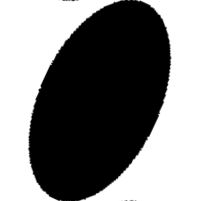
\includegraphics[scale=.5]{plots/fig1}
% \end{center}
\begin{center}
\newpage
Microscopic $\bfE$ field\\
\animategraphics[controls,scale=.6,palindrome]{6}{data/keep/e-lrem-}{1}{51}
\vfill
 
Microscopic Polarization\\
\animategraphics[controls,scale=.6,palindrome]{6}{data/keep/p-lrem-}{1}{51}

\vspace{2cm}

\end{center}

\subsection{Redo the Plots}

If for some reason you want to redo only the plots, like you changed a
line style, or frequency range, etc. do the following easy steps, so
you don not have to calculate unnecessary files.
\begin{enumerate}
\item Create a \verb=new= directory within PWD
\item \verb=PWD/hc> ls * > hoy=\label{deaqui}
\item \verb=PWD/new> mv ../hc/hoy .=
\item \verb=PWD/new> sort -tW -n -k 2 hoy > lista=\\after \verb=-t=
  put the identifier for the sorting, if any!
\item Edit \verb=lista= or \verb=hoy=, so you have the set you may want to redo the
  plots with. For instance select a few frequencies.
\item \verb=PWD/new> awk '{print "ln -s","../../hc/"$1,$1}' lista >lista2=
\item \verb=PWD/new> ./lista2=\\so now you have a symbolic link to the
  required files\label{aca}
\item Repeat from step \ref{deaqui} to  step \ref{aca} for directory \verb=res=
\item \verb=PWD/new> rm arrows/* plots/* movies/*=\\or any combination
  that you want to redo.
\item Run \verb=the-whole-enchilada.pl= just as you did the last time,
  and voil\`a!
\end{enumerate} 


\section{Internal Checkups}

\subsection{$\bfP\cdot\bfE$ approach}
As an internal check up we compare the reflectivity of Eq.~\ref{nir}
calculated through the macroscopic dielectric function $\bfge$, and
the Polarization $\bfP$. We recall that 
\begin{equation}\label{pol1}
\bfD(\bfr)=\bfE(\bfr)+4\pi\bfP(\bfr)=\bfge(\bfr)\cdot\bfE(\bfr)
,
\end{equation} 
we multiply by $\bfE(\bfr)$ to obtain
\begin{equation}\label{pol2}
\bfE(\bfr) \cdot\bfE(\bfr)
+4\pi\bfP(\bfr) \cdot\bfE(\bfr)=\bfge(\bfr)\cdot\bfE(\bfr) \cdot\bfE(\bfr)
,
\end{equation} 
working on principal axis $i$,
\begin{eqnarray}\label{pol3}
E_i^2(\bfr)
+4\pi P_i(\bfr)E_i(\bfr)&=&\ge_i(\bfr)E_i^2(\bfr)
\nonumber\\
P_i(\bfr)E_i(\bfr)
&=&\frac{1-\ge_i(\bfr)}{4\pi}E_i^2(\bfr)
.
\end{eqnarray}
Above can be calculated inside $(\ge_i(\bfr)=\ge_{bi})$
and outside $(\ge_i(\bfr)=\ge_{ai})$ the inclusion, since we know the
microscopic field $\bfE(\bfr)$ (in this case, along the principal
axis). Once we have $\bfP\cdot\bfE$ inside and outside the inclusion,
we can calculate the macroscopic $\ge_i^M$ as
\begin{equation}\label{pol4}
\ge_i^M=1+4\pi \left([P_i(\bfr)E_i(\bfr)]\Big|_{\bfr\,\in\,\mathrm{inclusion}}
+[P_i(\bfr)E_i(\bfr)]\Big|_{\bfr\,\notin\,\mathrm{inclusion}}\right)
,
\end{equation} 
from where we can calculate the reflectivity (Eq.~\ref{nir}).

In the following figure we show the comparison of the two methods,
from where we see a good agreement, confirming that the fields are
correctly calculated. We
do it for an elipse, and the details are found in 
\verb=programs/2torial/text/plots/A0=. In particular the file
\verb=pola.g= is used for the plot. We used a 201$\times$201 elipse
with $\ge_a$=Au, $ge_b=4$ and $N_H=100$.

\textcolor{red}{Warning}: This check muts be done by using the same
axis for every energy value. So, it is recommended to do it for
inclusions whose crystal axis are the same as the principal axis.
That is why we choose the elipse at 0$^\circ$. 

\begin{center}
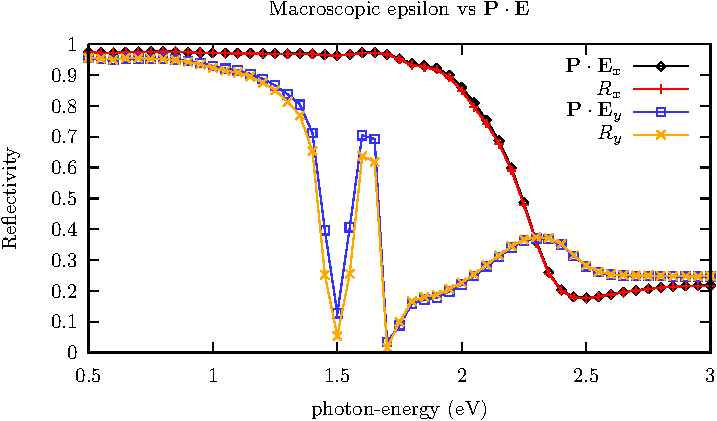
\includegraphics[scale=1]{plots/A0/pola}
\end{center}

\subsection{Dipolar Approximation}\label{dipole}

Following the notes of WLM (yet to be \LaTeX'ed), in the following
plots we compare the full approach (Haydock's) with the analytical
result of the Dipolar Field of an square array of cylindrical
inclusions. We obtain that for small $f$ both approaches are very
similar, whereas for large $f$, the dipolar field differs from the
full calculations, since the latter contains all different
multipoles. However, for large $f$ and low energy (high wavelength),
the dipolar field could be rather similar to the full field. We dare
the young soul to confirm such claim. 

\begin{center}
$f=0.117$ and $\hbar\go=2.05$ eV
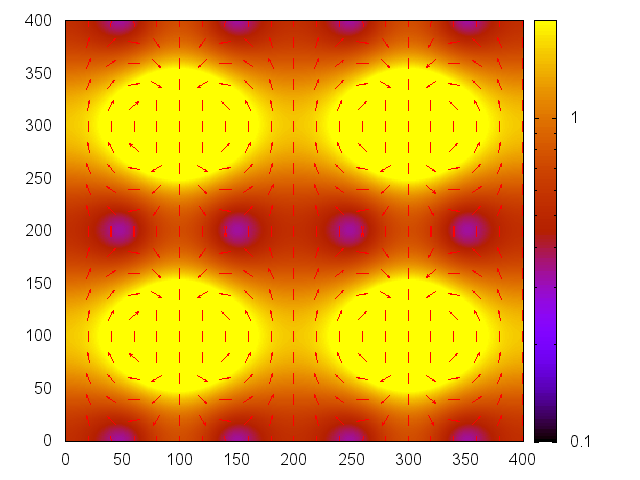
\includegraphics[scale=.31]{plots/manda/dipolar_W2.05_f.117}%
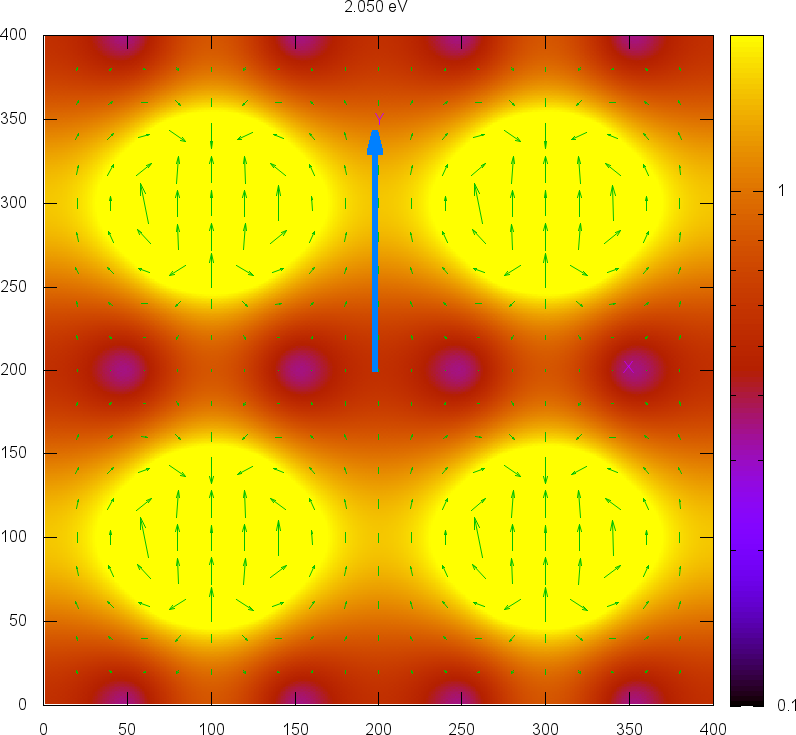
\includegraphics[scale=.2]{plots/manda/e-cilindro_A0.00_S1.000_f0.117_principal_0.00_ave_Nh_100_epsa_au_W2.050_epsb_8.000-0.000_dir_yp-dat.2x2}%
\end{center}
\newpage
\begin{center}
$f=0.269$ and $\hbar\go=1.95$ eV
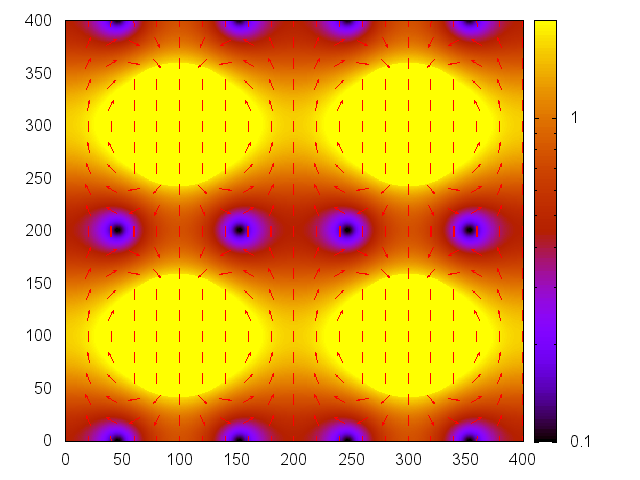
\includegraphics[scale=.31]{plots/manda/dipolar_W1.95_f.269}%
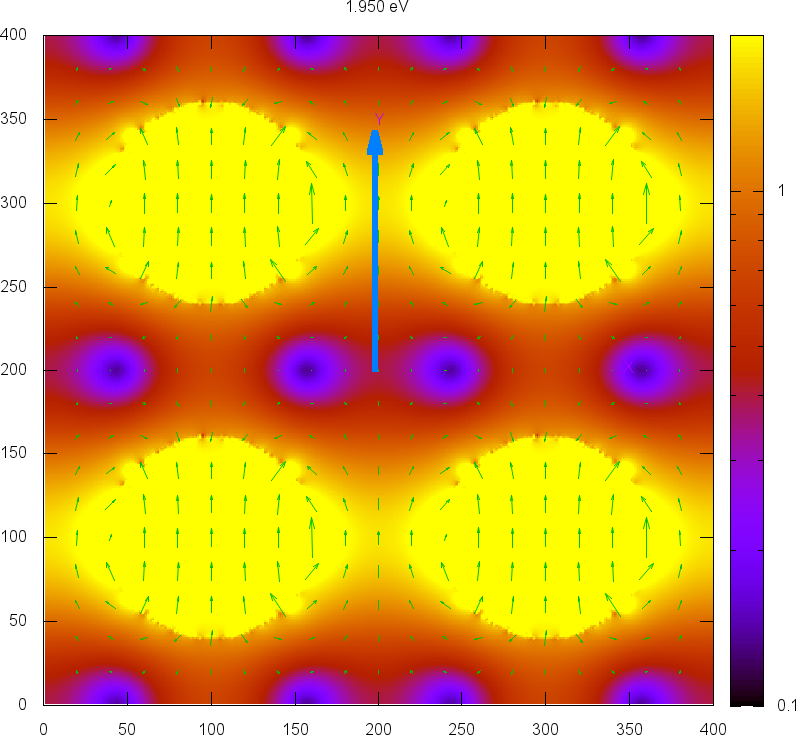
\includegraphics[scale=.2]{plots/manda/e-cilindro_A0.00_S1.000_f0.269_principal_0.00_ave_Nh_100_epsa_au_W1.950_epsb_8.000-0.000_dir_yp-dat.2x2}%
\end{center}

\begin{center}
$f=0.425$ and $\hbar\go=1.75$ eV
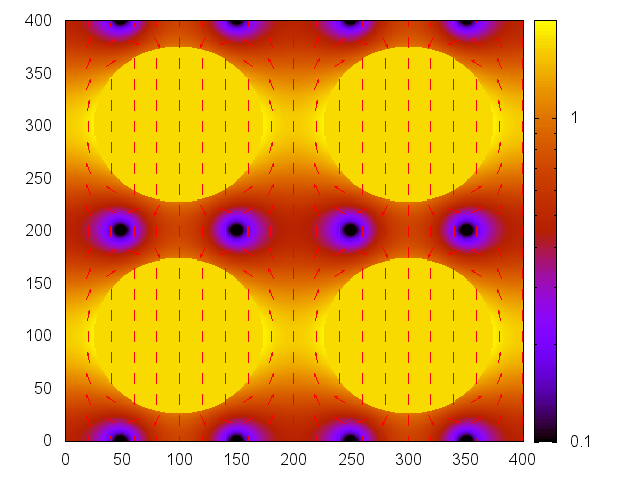
\includegraphics[scale=.31]{plots/manda/dipolar_W1.75_f.425}%
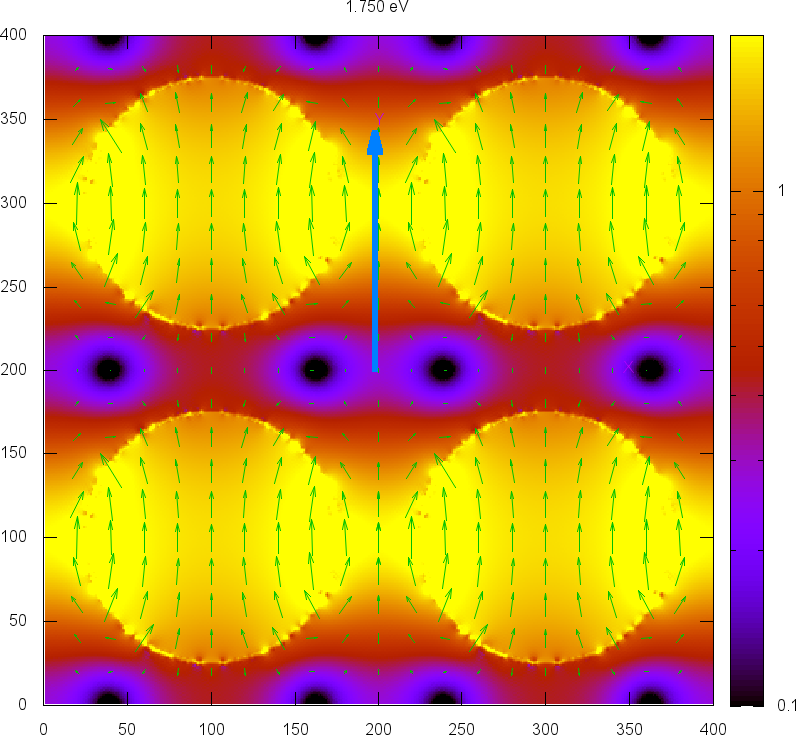
\includegraphics[scale=.2]{plots/manda/e-cilindro_A0.00_S1.000_f0.425_principal_0.00_ave_Nh_100_epsa_au_W1.750_epsb_8.000-0.000_dir_yp-dat.2x2}%
\end{center}
 

\section{Notes}
These are the notes for the calculation of the Fields as transcribed
by SP

\subsection{General theory}
\label{Theory}
We have shown how to get the macroscopic electromagnetic response of
composite systems 

We have propose an efficient homogenization procedure for the
calculation of optical properties of nanostructured composites.  we
use Eq.~(?) to obtain the optical properties of an
artificial binary crystal made of two materials $A$ and $B$ with
dielectric functions $\epsilon_A$ and $\epsilon_B$. We assume that
both media are local and isotropic so that $\epsilon_A$ and
$\epsilon_B$ are simply complex functions of the frequency.

We introduce the characteristic function $B(\mathbf r)$ of the
inclusions, such that $B(\mathbf r)\equiv1$ whenever $\mathbf r$ is on
the region $B$ occupied by the inclusions, and $B(\mathbf r)\equiv0$
otherwise. Thus, we may write the microscopic dielectric response as
\begin{equation}
  \label{epsmicro}
  \epsilon(\mathbf r)= 
  \frac{\epsilon_A}{u}\left( u-B(\mathbf r) \right),
\end{equation}
where we defined the spectral variable $u\equiv
1/(1-\epsilon_B/\epsilon_A)$ %\cite{Bergman}. 
The
longitudinal projection of Eq.~(\ref{epsmicro}) may be
written as
\begin{equation}
  \label{epsll}
  \hat \epsilon^{LL}_{\mathbf G\mathbf G'}= \frac{\epsilon_A}{u}\left(
    u- B ^{LL}_{\mathbf G\mathbf G'}\right),
\end{equation}
 According to Eq.~(\ref{}) we have to invert and take the $\mathbf
 0\mathbf 0$ element
\begin{equation}
  \label{epslli}
\left(  \hat \epsilon^{LL}_{\mathbf G\mathbf G'}\right)^{-1}_{\mathbf 0\mathbf 0}= 
  \frac{u}{\epsilon_A}\left(  u-
  B_{\mathbf G\mathbf G'}^{LL}\right)^{-1}_{\mathbf 0\mathbf 0}, 
\end{equation}

Now we have used the recursion relation
\begin{equation}\label{n+1}
  |\widetilde{n+1}\rangle\equiv \op H |n\rangle = b_{n+1}|n+1\rangle + a_n
  |n\rangle +   b_{n}|n-1\rangle, 
\end{equation}
where $\op H=B_{\mathbf G\mathbf G'}^{LL}$ and all the states
$|n\rangle$ are orthonormalized according to
\begin{equation}\label{ortonor}
  \langle n|m\rangle =  \delta_{nm},
\end{equation}
with $\delta_{nm}$ the Kronecker's delta function. The requirement of
orthonormality yields the generalized Haydock coefficients $a_n$,
$b_{n+1}$, given the previous coefficients $b_{n}$, and $a_{n-1}$. 

In the basis $\{|n\rangle\}$, $\op B$ is {\em represented} by a
tridiagonal matrix with $a_n$ along the main diagonal, $b_n$ along the
subdiagonal and $b_n$ along the supradiagonal, so that
\begin{equation}
\label{MWaveMatrix}
\left( u-\op B \right)\to \left(
\begin{array}{ccccc}
 u-a_0 & -b_1 & 0  & 0&\cdots\\
 -b_1 & u-a_1 & -b_2& 0& \cdots\\
 0   & -b_2 & u-a_2 & -b_3& \cdots\\
\vdots&\vdots&     &\vdots &\ddots
\end{array}
\right). 
\end{equation}

%where $\op B ^{LL}$ is the Fourier transform of the characteristic
%function $B(\mathbf r)$ .


According to Eq. (?), we do not require the full
inverse of the matrix (?), but only the element in the
first row and first column. Following Ref. \verb=\cite{Mochan3}=, we obtain
that element as a continued fraction, which substituted into
Eq. (?) yields
\begin{equation}\label{chin}
  \left( \epsilon^{M}_{LL}\right)^{-1} = \frac{u}{\epsilon_A} \frac{1} {u-a_0 -\frac{
      b_1^2} {u -a_1 -\frac{b_2^2} {u- a_2 -\frac{b_3^2}{\ddots }}}}.
\end{equation}


%\section{Recursive method }
%\label{HaydockMethod} 

The constitutive equation in the long wavelength limit is
\begin{equation}
\label{constitutiva}
  \mathbf D_{L} = \hat \epsilon_{LL} \mathbf E_L,
\end{equation}
so electric field is
\begin{equation}\label{EL}
  \mathbf E_L = (\hat\epsilon_{LL})^{-1}\mathbf D_L.
\end{equation}
Averaging  $\mathbf E_L $ we get
\begin{equation}\label{ELp}
  \mathbf E_L^a = (\hat\epsilon_{LL})_{aa}^{-1}\mathbf D_L^a +
  (\hat\epsilon_{LL})_{af}^{-1}\mathbf D_L^f,
\end{equation}
but $\mathbf D_L$ has not fluctuations, $\mathbf D_L^f=
\hat{\mathcal{P}}_{f} \mathbf D_L=\mathbf 0$. So
\begin{equation}\label{ELM}
  \mathbf E_L^a = (\hat\epsilon_{LL})_{aa}^{-1}\mathbf D_L^a.
\end{equation}
or
\begin{equation}\label{ELMm}
  \mathbf E_L^M = (\hat\epsilon_{LL})_{aa}^{-1}\mathbf D_L^M.
\end{equation}


In the basis $\{|n\rangle\}$, $\mathbf D^L$ is different of zero only
in the first position,
\begin{equation}
\label{dl}
 \mathbf D_L \to
\left(
\begin{array}{c}
 \mathbf D_0 \\
 \mathbf 0 \\ 
 \vdots\\
 \mathbf 0 \\ 
\end{array}
\right). 
\end{equation}
 but $\mathbf E^L$  is a vector of the form
\begin{equation}
\label{el}
 \mathbf E_L \to
\left(
\begin{array}{c}
 \mathbf E_0 \\
 \mathbf E_1 \\ 
 \vdots\\
 \mathbf E_N \\ 
\end{array}
\right). 
\end{equation}
So
\begin{equation}
\label{consti}
\left(
\begin{array}{c}
 \mathbf D_0 \\
 \mathbf 0 \\ 
 \vdots\\
 \mathbf 0 \\ 
\end{array}
\right) = \frac{\epsilon_A}{u}
 \left(
\begin{array}{cccccc}
 u-a_0 & -b_1 & 0  & 0&\cdots & 0  \\
 -b_1 & u-a_1 & -b_2& 0& \cdots &0\\
 0   & -b_2 & u-a_2 & -b_3& \cdots &0\\
\vdots&\vdots& \vdots    &\vdots &\ddots &\vdots\\
 0  & 0 &0  &   0 & -b_{N-1}  & u-a_N
\end{array}
\right). 
\left(
\begin{array}{c}
 \mathbf E_0 \\
 \mathbf E_1 \\ 
 \vdots\\
 \mathbf E_N \\
\end{array}
\right). 
\end{equation}
therefore
\begin{equation}
-b_N \mathbf E_{N-1}  +(u-a_N)\mathbf E_N=0
\end{equation}
and gives for the last row
\begin{equation}
 \mathbf E_{N-1}=\frac{u-a_N}{b_N}\mathbf E_N.
\end{equation}
In general,
\begin{equation}
-b_n \mathbf E_{n-1} +(u-a_n)\mathbf E_n=b_{n+1}\mathbf E_n=0
\end{equation}
so
\begin{equation}
 \mathbf E_{n-1}=\frac{(u-a_n)\mathbf E_N-b_{n+1}\mathbf E_{n+1}}{b_n}
\end{equation}
and finish as
\begin{equation}
(u-a_0)\mathbf E_0 -b_{1}\mathbf E_1=\frac{u}{\epsilon_A}\mathbf D_0
\end{equation}
cuidado, son vectores
but
\begin{equation}
(u-a_0) -b_{1}\mathbf E_1/\mathbf E_0=\frac{u}{\epsilon_A}\mathbf
  D_0/\mathbf E_0\equiv \frac{u}{\epsilon_A}\epsilon^M
\end{equation}
and the microscopic field can be obtained as
\begin{equation}
\mathbf E_{\mathbf G}=\sum_n \mathbf E_n \hat {\mathbf G }
\phi_n(\mathbf G)
\end{equation}
where $\mathbf \phi_n(\mathbf G)=\langle\mathbf{ G}|n \rangle$, so
\begin{equation}
\mathbf E (\mathbf r)=\mathscr{F}^{-1}\{\mathbf E_{\mathbf G} \}
\end{equation}

\section{Optical Activity}

\subsection{Diagonalization}
The eigenvalues and eigenvectors of a $2\times 2$ symmetric (complex) matrix
$M\ket{\lambda_i}=\lambda_i\ket{\lambda_i}$, are obtained as follows. Let
\begin{equation}\label{h.1}
M=\left(\begin{array}{cc} 
M_{xx}&M_{xy}\\ 
M_{xy}&M_{yy}
\end{array}\right)
.
\end{equation} 
Then,
\begin{eqnarray}\label{h.29}
\left|\begin{array}{cc}
M_{xx}-\lambda&M_{xy}\\
M_{xy}&M_{yy}-\lambda
\end{array}\right|
&=&(M_{xx}-\lambda)(M_{yy}-\lambda) -M^2_{xy}
\nonumber\\
&=&
\lambda^2-\lambda(M_{xx}+M_{yy})+M_{xx}M_{yy}-M^2_{xy}
\nonumber\\
&=&
\lambda^2-\lambda 
\mathrm{Tr}[M]
+
\mathrm{Det}[M]
=0
\nonumber\\
\to\lambda_{\pm}&=&
\frac{1}{2}\left(
\mathrm{Tr}[M]
\pm\sqrt{(\mathrm{Tr}[M])^2-4 \mathrm{Det}[M]}
\right)
.
\end{eqnarray}
The eigenvectors follow from
\begin{eqnarray}\label{h.1}
\left(\begin{array}{cc}
M_{xx}-\lambda&M_{xy}\\
M_{xy}&M_{yy}-\lambda
\end{array}\right)
\left(\begin{array}{c}
c\\
c
\end{array}\right)
&=&0
\nonumber\\
(M_{xx}-\lambda)c+M_{xy}d&=&0
\nonumber\\
M_{xy}c+(M_{yy}-\lambda)d&=&0
\nonumber\\
\to d&=&\frac{\lambda-M_{xx}}{M_{xy}}c,
\nonumber\\
\to
 \bfV
&=&
\frac{c}{M_{xy}}\left(\begin{array}{c}
M_{xy}\\
\lambda-M_{xx}
\end{array}\right)
,
\end{eqnarray}
and use $c$ to normalize the vector, then
\begin{equation}\label{h.3}
 \bfv_\pm
=
\frac{1}{\sqrt{|M_{xy}|^2+|\lambda_\pm-M_{xx}|^2}}
\left(\begin{array}{c}
M_{xy}\\
\lambda_\pm-M_{xx}
\end{array}\right)
,
\end{equation}
with $\bfv_\pm\cdot\bfv_\pm^T=1$,
and $\bfv_\mp\cdot\bfv_\pm=0$ can be easily verified for the case of
real $M$. If $M$ is complex the complex eigenvectors are not
necessarily perpendicular in the standard sense (see \ref{app}).  

\subsection{Elliptical Polarization}

To obtain the corresponding ellipse that represents the polarization
of the Electric field, we proceed as follows.

We take any one of the $\bfv_{\pm}$ (complex) eigenvectors, and write it as
\begin{equation}\label{w.1}
\vec v=\vec v'+i\vec v''
,
\end{equation} 
then, the electric field is
\begin{equation}\label{w.2}
\bfE(t)\propto \vec v'\cos\omega t+\vec v''\sin\omega t
.
\end{equation}
Taking the components
\begin{eqnarray}\label{w.3}
E_x&=&v'_x\cos\omega t+v''_x\sin\omega t
\nonumber\\
E_y&=&v'_y\cos\omega t+v''_y\sin\omega t
,
\end{eqnarray}
and 
eliminating $\cos\omega t$ and 
$\sin\omega t$, respectively, we obtain
\begin{eqnarray}\label{w.4}
v'_y E_x-v'_x E_y&=&(v'_y v''_x-v'_x v''_y)\sin\omega t
\nonumber\\
v''_y E_x-v''_x E_y&=&(v''_y v'_x-v''_x v'_y)\cos\omega t
,
\end{eqnarray}
from where we obtain
\begin{eqnarray}\label{w.5}
\sin\omega t&=&\frac{v'_y E_x-v'_x E_y}{v'_y v''_x - v'_x v''_y}
\nonumber\\
\cos\omega t&=&-\frac{v''_y E_x-v''_x E_y}{v'_y v''_x - v'_x v''_y}
.
\end{eqnarray}
Using $\cos^2x+\sin^2x=1$, we can eliminate the time by writing
\begin{equation}\label{w.6}
\vec E^T M \vec E=1
,
\end{equation}
where we write
$\vec E$ as a column vector and $M$ is a matrix with components
\begin{eqnarray}\label{w.8}
	   M_{xx}&=&|v_y|^2/D
\nonumber\\
	   M_{xy}&=&-(v'_x v'_y+v''_x v''_y)/D
\\
M_{yy}&=&|v_x|^2/D
,
\end{eqnarray}
with
\begin{equation}\label{w.9}
D=(v'_y v''_x-v'_x v''_y)^2
.
\end{equation}
The secular equation follows from Eq.~\eqref{h.29},
\begin{equation}\label{w.39}
\lambda^2 -\lambda \mathrm{tr}(M) + \mathrm{det}(M)=0
,
\end{equation}
with solutions
\begin{equation}\label{h.56}
\lambda_\pm=\big(\mathrm{tr}(M)\pm\sqrt{\mathrm{tr}(M)^2-4\mathrm{det}(M)}\big)/2
,
\end{equation}
with the corresponding
eigenvectores $|+\rangle$ and $|-\rangle$ (not to be confused with
right-left circularly polarizations).
Writing $\vec E=E_+|+\rangle + E_-|-\rangle$ we obtain
\begin{equation}\label{w.51}
\vec E^T M \vec E=\lambda_- E_-^2 + \lambda_+ E_+^2 = 1
,
\end{equation}
that is the equation of an ellipse with semi-major $a$ and semi-minor
$b$ axis given by
\begin{eqnarray}\label{w.69}
a&=&\frac{1}{\sqrt{\lambda_-}}
\\
b&=&\frac{1}{\sqrt{\lambda_+}}
.
\end{eqnarray}
The directions {\textcolor{red}{\it with respect to the crystal $x$ axis}} are given by
\begin{eqnarray}\label{w.70}
\tan\alpha_-&=&\frac{\lambda_- - M_{xx}}{M_{xy}}
\\
\tan\alpha_+&=&\frac{\lambda_+ - M_{xx}}{M_{xy}}
,
\end{eqnarray}
with $\alpha_+$ and $\alpha_-$ real angles perpendicular to each other
(we are using the same notation as M\& M PRB {\bf 85}, 125418 (2012)).
The helicity of the polarization ellipse is given by the sign of
\begin{eqnarray}\label{w.89}
\mathrm{Re}[\bfv_\pm]\times\mathrm{Im}[\bfv_\pm]
&=&
(v_x'\hat x+v_y'\hat y)
\times
(v_x''\hat x+v_y''\hat y)
=(v_x'v_y''-v_x''v_y')\hat z
\nonumber\\
\to \mathrm{sgn}[v_x'v_y''-v_x''v_y']
&=&\left\{\begin{array}{cl}
-&\circlearrowright\mathrm{left-polarized}
\\ 
+&\circlearrowleft\mathrm{right-polarized}
\end{array}\right.
\end{eqnarray}

Above is implemented in
\verb=fracCont.pl,corre-principal-axes.pl,haydock2DNRBase.pl=. Also
there is \verb=gnuplot= program \verb=semiejes.g= where above is
implemented for any $\bfv$ of the form given by Eq.~\eqref{w.1}.

\appendix
\section{Complex Eigenvectors}\label{app}
After WLM, we show that $\Theta_1-\Theta_2=\pi/2$, where 
$\Theta_\ga=\theta_\ga+i\mathrm{Im}(\Theta_\ga)$.
We have that
\begin{eqnarray}\label{wlm.1}
V_1^T\cdot\ge\cdot V_2
&=&
V_1^T\cdot\big(\ge\cdot V_2\big)
=
\lambda_2V_1^T\cdot V_2\to\mathrm{scalar}=\mathrm{scalar}^T
\nonumber\\
&=&
(V_1^T\cdot\ge\cdot V_2)^T
=
V_2^T\cdot\ge\cdot V_1
=
\lambda_1
V_2^T\cdot V_1
=
\lambda_1
(V_2^T\cdot V_1)^T
=
\lambda_1
V_1^T\cdot V_2
\nonumber\\
\big(\lambda_1-\lambda_2\big)
V_1^T\cdot V_2
&=&
0
\Rightarrow
V_1^T\cdot V_2=0
.
\end{eqnarray}
Thus the eigenvectors are perpendicular, within the Euclidean metric,
even if the eigenvalues, $\lambda_{1,2}$, are complex.
Then, it follows that
$\Theta_1-\Theta_2=\pi/2$,
 even if the angles, $\Theta_{1,2}$, are  complex. 
But if $\Theta_1-\Theta_2=\pi/2$, the complex part of $\Theta_1$ must
be equal to the complex part of $\Theta_2$, and then
$\theta_1-\theta_2=\pi/2$.  
Indeed, we have confirmed numerically that
$\mathrm{Im}(\Theta_1)=\mathrm{Im}(\Theta_2)$, and that
$\theta_1-\theta_2=\mathrm{sgn}(\theta_1-\theta_2)\pi/2$.

\section{Projection of the Electric Field}

We can calculate the electric field $\bfE(\bfr)$ as follows. We begin
by using two mutually perpendicular polarizations, $\bfgvare_{1,2}$ for the external
(unitary) field $\bfE_\mathrm{ext}$, say along the crystal axis $x$ and $y$,
then we can write,
\begin{eqnarray}\label{ee.1}
\bfE(\bfr;\bfgvare_1)
&=&
E_x(\bfr;\bfgvare_1)\hat x
+
E_y(\bfr;\bfgvare_1)\hat y
\quad \mathrm{for}\quad\bfE_\mathrm{ext}=\bfgvare_1=\hat x 
\nonumber\\
\bfE(\bfr;\bfgvare_2)
&=&
E_x(\bfr;\bfgvare_2)\hat x
+
E_y(\bfr;\bfgvare_2)\hat y
\quad \mathrm{for}\quad\bfE_\mathrm{ext}=\bfgvare_2=\hat y 
,
\end{eqnarray}
where $\bfE(\bfr;\bfgvare_{i})$ is the microscopic field for
$\bfE_\mathrm{ext}=\bfgvare_i$. 
We want to express $\bfE(\bfr;\bfgvare_{i})$ along any given direction
$\hat\bfv$, then
\begin{eqnarray}\label{ee.2}
\bfE(\bfr;\hat\bfv)
&=&
(\bfE(\bfr;\bfgvare_{i})\cdot\hat\bfv)\hat\bfv
=
(\bfE(\bfr;\bfgvare_{i})\cdot\hat\bfv)(\hat v_x\hat x+\hat v_y\hat y)
\nonumber\\
&=&
 (\hat v_xE_x(\bfr;\bfgvare_{i})
+
\hat v_yE_y(\bfr;\bfgvare_{i}))
 (\hat v_x\hat x+\hat v_y\hat y)
\nonumber\\
&=&
E_x(\bfr;\hat\bfv)\hat x
+
E_y(\bfr;\hat\bfv)\hat y
\nonumber\\
E_x(\bfr;\hat\bfv)&=&
 (\hat v_xE_x(\bfr;\bfgvare_{i})
+
\hat v_yE_y(\bfr;\bfgvare_{i}))\hat v_x
\nonumber\\
E_y(\bfr;\hat\bfv)&=&
 (\hat v_xE_x(\bfr;\bfgvare_{i})
+
\hat v_yE_y(\bfr;\bfgvare_{i}))\hat v_y
,
\end{eqnarray} 
\section{Ellipses}

\Verb+corre-angles.pl --od=plots/ --idf=meps/eps-*-dat --tam=.1+
\Verb+corre-arrows.pl --od=arrows/ --idf=meps/eps-*-dat --tam=.1+
\Verb+corre-elipses.pl --od=movies/ --scale=1.250 --angle=24 --Nh=100+
\Verb+--epsa=ag --epsb=1.001 --axes=principal -nem=vsw --ep=e+

%\Verb+corre-angles.pl --od=plots/
%--idf=meps/eps-cross_A24.00_S1.250_f0.592_crystal_Nh_100_epsa_ag_epsb_1.001-0.000-dat
%--tam=.1+

%\Verb+corre-arrows.pl --od=arrows/
%--idf=meps/eps-cross_A24.00_S1.250_f0.592_crystal_Nh_100_epsa_ag_epsb_1.001-0.000-dat
%--tam=.1+

%\Verb+corre-elipses.pl --od=movies/ --scale=1.250 --angle=24 --Nh=100 --epsa=ag --eps%b=1.001 --axes=principal -nem=vsw --ep=e+

\vspace{2cm}
\begin{center}

\includegraphics[scale=.5]{thatsallfolks}
\end{center}

\end{document}

Por cierto, lo de los ?ngulos creo que viene de que epsilon es una                 
matriz sim?trica a?n cuando es compleja (en este caso en que no hay                
dispersi?n espacial, aunque no estoy seguro de por qu?). La                        
amplitud de reflexi?n r es entonces tambi?n una matriz sim?trica. Entonces         
si v_1 y v_2 son eigenvectores columna, v_1^T.r.v_2=v_1^T.(r.v_2)=lambda_2         
v_1^T.v_2= (v_1^T.r.v_2)^T=v_2^T.r^T.v_1=v_2^T.r.v_1=lambda_1                      
v_2^T.v_1=lambda_1 v_1^T.v_2, con lambda los eigenvalores. Luego,                  
(lambda_2-lambda_1)v_1^T.v_2=0 y los eigenvectores son perpendiculares             
(con la m?trica euclideana) aunque los eigenvalores sean                           
complejos. Luego, la resta de ?ngulos vale pi/2, aunque sean                       
complejos. S?lo me falta acabar de entender c?mo se definen los                    
?ngulos complejos. 


It seems that if the eigenvectors of the diagonalization are complex,
this could mean optical activity. Then, we show the elipse that would
represent the elliptical polarization, that is obtained as follows.
Let $\bfV_{1,2}$ represent the two eigenvectors corresponding to the two
eigenvalues $\lambda_{1,2}$, which we identify as the values of the
macroscopic dielectric function along the principal directions 1 and
2. Write
\begin{eqnarray}\label{vecs}
\bfV_{\ga}&=&v_{\ga,x}\hat\bfx+v_{\ga,y}\hat\bfy\quad(\ga=1,2)
\nonumber \\
&=&
(v^{\rmr}_{\ga,x}+iv^{\rmi}_{\ga,x})
\hat\bfx+
(v^{\rmr}_{\ga,y}+iv^{\rmi}_{\ga,y})
\hat\bfy
\nonumber \\
&=&
(v^{\rmr}_{\ga,x}\hat\bfx+v^{\rmr}_{\ga,y}\hat\bfy)
+
i(v^{\rmi}_{\ga,x}\hat\bfx+v^{\rmi}_{\ga,y}\hat\bfy)
.
\end{eqnarray}
The angle of the principal directions
is give as
\begin{eqnarray}\label{teta}
\theta_\ga
&=&
\mathrm{Re}\left[\tan^{-1}\left(\frac{v_{\ga,y}}{v_{\ga,x}}\right)\right]
\nonumber\\
\frac{v_{\ga,y}}{v_{\ga,x}}&=&
\frac{v_{\ga,y}v^*_{\ga,x}}{|v_{\ga,x}|^2}
=
\frac{(v^\rmr_{\ga,y}+i v^\rmi_{\ga,y})(v^\rmr_{\ga,x}-i v^\rmi_{\ga,x})}{|v_{\ga,x}|^2}
\nonumber\\
&=&
\frac{1}
{|v_{\ga,x}|^2}
\Big(
v^\rmr_{\ga,y}v^\rmr_{\ga,x}
+
v^\rmi_{\ga,y}y^\rmi_{\ga,x}
+i
(
v^\rmi_{\ga,y}v^\rmr_{\ga,x}
-
v^\rmr_{\ga,y}y^\rmi_{\ga,x}
)
\Big)
,
\end{eqnarray}
where $\theta_1+\theta_2=\pi/2$. The elliptical polarization is represented
by an elipse with a semiaxis $a_\ga$ (along $\theta_{\ga}$) and semiaxis $b_\ga$, both scaled
according to
\begin{equation}\label{eli}
{\cal E}_\ga\to(a_\ga,b_\ga)=
(e^\rmr_\ga,e^\rmi_\ga)/e_\ga
%\left\{
%\begin{array}{cc}
%(1,e^\rmi_\ga/e^\rmr_\ga)&\mathrm{if}\, e^\rmr_\ga>e^\rmi_\ga\\
 %(e^\rmr_\ga/e^\rmi_\ga,1)&\mathrm{if}\, e^\rmr_\ga<e^\rmi_\ga
 %\end{array}
%\right.
,
\end{equation}  
where
\begin{eqnarray}\label{es}
e^\rmr_\ga&=&\sqrt{(v^{\rmr}_{\ga,x})^2+(v^{\rmr}_{\ga,y})^2}
\\
e^\rmi_\ga&=&\sqrt{(v^{\rmi}_{\ga,x})^2+(v^{\rmi}_{\ga,y})^2}
\\
e_\ga&=&\sqrt{(e^{\rmr}_{\ga})^2+(e^{\rmi}_{\ga})^2}
.
\end{eqnarray}
If $e^\rmi_\ga=0$, ${\cal
  E}_{1,2}$ are straight lines at angles $\theta_{1,2}$ perpendicular
to each other.

Above is implemented in \verb=fracCont.pl,corre-principal-axes.pl,haydock2DNRBase.pl=

We define $\eta_\ga$, known as the {\it third flattening} in the argot of
the ellipses, as
\begin{equation}\label{eta}
\eta_\ga\equiv \frac{a_\ga-b_\ga}{a_\ga+b_\ga}
,
\end{equation} 
that goes from 1 to -1 as the go from a flat ellipse along $\theta_1$
to a flat ellipse along $\theta_2$, and when $\eta_\ga=0$ we have
circular polarization. The plots of $\eta_\ga$ are also implemented in 
\verb=the-whole-enchilada.pl=.


Roubaix armadillo elite

Por cierto, hay un paquete PDL::IO::Storable, que, hasta donde                   
entend?, es como PDL::IO::Dumper, nuestro superpaquete para leer y               
escribir estructuras complejas con PDL's, pero en binario. Tal vez eso           
nos pueda ahorrar mucho tiempo. Parece que jala en la ?ltima versi?n             
de PDL pero no jalaba en las anteriores. Hay que probar.                         
                                                                                 
Saludos,                                                                         
Luis 
